% Prof. Dr. Ausberto S. Castro Vera
% UENF - CCT - LCMAT - Curso de Ci\^{e}ncia da Computa\c{c}\~{a}o
% Campos, RJ,  2022
% Disciplina: Paradigmas de Linguagens de Programa\c{c}\~{a}o
% Aluno: Rômulo Souza Fernandes



\chapter{ Aplica\c{c}\~{o}es da Linguagem Python}

Neste capítulo será apresentada 5 aplicações completas na linguagem de programação Python, com base nos autores \cite{Perkovic2016}, \cite{Borges2014}, \cite{Severance2016} e \cite{Lutz2007}. Cada caso contém:
\begin{itemize}
  \item Uma breve descri\c{c}\~{a}o da aplica\c{c}\~{a}o
  \item O c\'{o}digo completo da aplica\c{c}\~{a}o,
  \item Imagens do c\'{o}digo fonte no compilador-interpretador,
  \item Imagens dos resultados ap\'{o}s a compila\c{c}\~{a}o-interpreta\c{c}\~{a}o do c\'{o}digo fonte
  \item Links e referencias bibliogr\'{a}ficas de onde foi obtido a aplica\c{c}\~{a}o
\end{itemize}




    \section{Opera\c{c}\~{o}es b\'{a}sicas}
    
    O código a seguir apresenta algumas operações básicas da matemática que podem ser feitas na linguagem Python, como adição, subtração, multiplicação e divisão. Essas operações serão escolhidas em um menu de opções. 
	\begin{lstlisting}
# Autor: Romulo Souza Fernandes
# E-mail: 00119110559@pq.uenf.br
# Data de criacao: 28/10/22
# Ciencia da Computacao - UENF
# Disciplina: PLP
		
		
continuar_usando = "SIM"
		
while continuar_usando == "SIM":
 # Criando um menu de opcoes
 print("SELECIONE A OPERAcaO DESEJADA")
 print("+ para Adicao")
 print("- para Subtracao")
 print("* para Multiplicacao")
 print("/ para Divisao")
		
 # Interacao com o usuario
 operacao = input("\nQual operacao voce deseja realizar? ")
		
 # Criando as operacoes e as apresentacoes de respostas
		
 # Adicao
 if operacao == "+":
  a1 = float(input("\nDigite o primeiro valor: "))
  a2 = float(input("Digite o segundo valor: "))
  adicao = a1 + a2
  print("\nA soma entre", a1, "e", a2, "e:", adicao, "\n")
  print("*"*33, "\n")
  continuar_usando = input("Gostaria de fazer outra operacao? 
  ").upper()
  print("*"*33, "\n")
		
 # Subtracao
 if operacao == "-":
  b1 = float(input("\nDigite o primeiro valor: "))
  b2 = float(input("Digite o segundo valor: "))
  subtracao = b1 - b2
  print("\nA subtracao entre", b1, "e", b2, "e:", subtracao,
   "\n")
  print("*"*33, "\n")
  continuar_usando = input("Gostaria de fazer outra operacao?
   ").upper()
  print("*"*33, "\n")
		
 # Multiplicacao
 if operacao == "*":
  c1 = float(input("\nDigite o primeiro valor: "))
  c2 = float(input("Digite o segundo valor: "))
  multiplicacao = c1 * c2
  print("\nA multiplicacao entre", c1,
  "e", c2, "e:", multiplicacao, "\n")
  print("*"*33, "\n")
  continuar_usando = input("Gostaria de fazer outra operacao?
   ").upper()
  print("*"*33, "\n")
		
 # Divisao
 if operacao == "/":
  d1 = float(input("\nDigite o primeiro valor: "))
  d2 = float(input("Digite o segundo valor: "))
  while d2 == 0:  # Garantindo que d2 nao seja zero!!
  print("O segundo valor nao pode ser zero!")
  d2 = float(input("\nDigite o segundo valor (diferente 
  de zero): "))
  divisao = d1 / d2
  print("\nA divisao entre", d1, "e", d2, "e:", divisao, "\n")
  print("*"*33, "\n")
  continuar_usando = input("Gostaria de fazer outra operacao?
   ").upper()
  print("*"*33, "\n")
	\end{lstlisting}

	Como vemos no código, inicialmente uma variável chamada "continuar\textunderscore usando", é criada e definida como "SIM". Na estrutura de repetição While, enquanto a variável "continuar\textunderscore usando", for igual a "SIM", o laço continuará. Um menu de interação é criado dentro desse While, o menu oferece as seguintes opções de escolha, soma, subtração, multiplicação e divisão. A variável chamada "operação" tem a função de receber e guardar a opção desejada pelo usuário. Caso a opção escolhida seja "+", a operação de soma será realizada, apresentará o resultado e também irá perguntar se o usuário deseja continuar usando, caso a respostar não seja "SIM", o programa irá finalizar, funcionando da mesma forma para as outras operações, caso forem escolhidas. A seguir temos algumas imagens demonstrando o código de operações básicas rodando no Visual Studio Code.

	\begin{figure}[H]
		\begin{center}
			\caption{Opção adição} \label{ling1}
			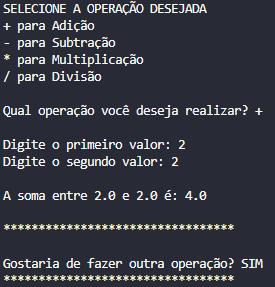
\includegraphics[width=5cm]{soma.PNG} \\
			{\tiny \sf Fonte:{ Autor}}
		\end{center}
	\end{figure}

	\begin{figure}[H]
		\begin{center}
			\caption{Opção subtração} \label{ling1}
			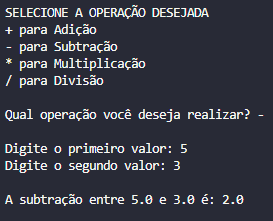
\includegraphics[width=5cm]{subtracao.PNG} \\
			{\tiny \sf Fonte:{ Autor}}
		\end{center}
	\end{figure}

	\begin{figure}[H]
		\begin{center}
			\caption{Opção multiplicação} \label{ling1}
			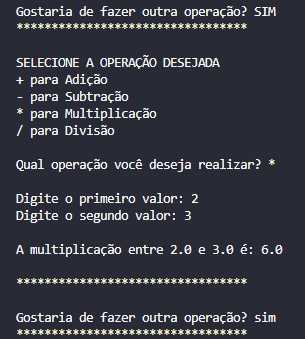
\includegraphics[width=5cm]{multi.PNG} \\
			{\tiny \sf Fonte:{ Autor}}
		\end{center}
	\end{figure}
	
	\begin{figure}[H]
		\begin{center}
			\caption{Opção divisão} \label{ling1}
			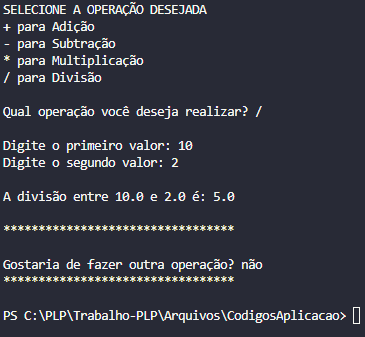
\includegraphics[width=5cm]{divisao.PNG} \\
			{\tiny \sf Fonte:{ Autor}}
		\end{center}
	\end{figure}
	
	
    \section{Programas gr\'{a}ficos}
     O código a seguir apresenta
	\begin{lstlisting}
# Autor: Romulo Souza Fernandes
# E-mail: 00119110559@pq.uenf.br
# Data de criacao: 28/10/22
# Ciencia da Computacao - UENF
# Disciplina: PLP


# Importando todo conteudo do Tkinter
from tkinter import *

# Classe que exibe os controles na tela


class Application:
	def __init__(self, master=None):
		# Criacao do primeiro container, chamado widget1
		self.widget1 = Frame(master)
		# Informando o gerenciador de geometria pack
		self.widget1.pack()
		# Utilizando o widget label para imprimir na tela
		self.msg = Label(self.widget1, text="Primeiro
		 widget")
		self.msg["font"] = ("Verdana", "10", "italic",
		 "bold")
		self.msg.pack()
		self.sair = Button(self.widget1)
		self.sair["text"] = "Sair"
		self.sair["font"] = ("Calibri", "10")
		self.sair["width"] = 5
		self.sair["command"] = self.widget1.quit
		self.sair.pack()


# Instanciando a classe TK()
# Ela permite que os widgets sejam utilizados na aplicacao
root = Tk()

# Passando a variavel root como parametro do metodo
# construtor da classe Application
Application(root)

# Chamada do metodo para exibir na tela
root.mainloop()
	\end{lstlisting}
	A seguir temos algumas imagens demonstrando o código do programa gráfico rodando no Visual Studio Code.


    \section{Programas com Objetos}
    O código a seguir apresenta
\begin{lstlisting}
# Autor: Romulo Souza Fernandes
# E-mail: 00119110559@pq.uenf.br
# Data de criacao: 28/10/22
# Ciencia da Computacao - UENF
# Disciplina: PLP

class Pessoa:
def __init__(self, nome: str, idade: int, altura: float):
self.nome = nome
self.idade = idade
self.altura = altura

def dizer_ola(self):
print(f'Ola, meu nome e {self.nome}. Tenho {self.idade} '
f'anos e minha altura e {self.altura}m.')

def cozinhar(self, receita: str):
print(f'Estou cozinhando um(a): {receita}')

def andar(self, distancia: float):
print(f'Sai para andar. Volto quando completar {distancia} metros')


# Instancia um objeto da Classe "Pessoa"
pessoa = Pessoa(nome='Joao', idade=25, altura=1.88)

# Chama os metodos de "Pessoa"
pessoa.dizer_ola()
pessoa.cozinhar('Spaghetti')
pessoa.andar(750.5)
\end{lstlisting}
	A seguir, uma imagem demonstrando o código utilizando objetos no Python, rodando no Visual Studio Code.
    \begin{figure}[H]
    	\begin{center}
    		\caption{Opção divisão} \label{ling1}
    		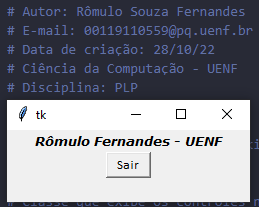
\includegraphics[width=7cm]{grafico.PNG} \\
    		{\tiny \sf Fonte:{ Autor}}
    	\end{center}
    \end{figure}
    
    \section{O algoritmo Quicksort}
    O código a seguir apresenta
\begin{lstlisting}
# Autor: Romulo Souza Fernandes
# E-mail: 00119110559@pq.uenf.br
# Data de criacao: 28/10/22
# Ciencia da Computacao - UENF
# Disciplina: PLP

# Python program for implementation of Quicksort Sort

# This implementation utilizes pivot as the last element in the nums list
# It has a pointer to keep track of the elements smaller than the pivot
# At the very end of partition() function, the pointer is swapped with the pivot
# to come up with a "sorted" nums relative to the pivot


# Function to find the partition position
def partition(array, low, high):

# choose the rightmost element as pivot
pivot = array[high]

# pointer for greater element
i = low - 1

# traverse through all elements
# compare each element with pivot
for j in range(low, high):
if array[j] <= pivot:

# If element smaller than pivot is found
# swap it with the greater element pointed by i
i = i + 1

# Swapping element at i with element at j
(array[i], array[j]) = (array[j], array[i])

# Swap the pivot element with the greater element specified by i
(array[i + 1], array[high]) = (array[high], array[i + 1])

# Return the position from where partition is done
return i + 1

# function to perform quicksort


def quickSort(array, low, high):
if low < high:

# Find pivot element such that
# element smaller than pivot are on the left
# element greater than pivot are on the right
pi = partition(array, low, high)

# Recursive call on the left of pivot
quickSort(array, low, pi - 1)

# Recursive call on the right of pivot
quickSort(array, pi + 1, high)


data = [1, 7, 4, 1, 10, 9, -2]
print("Unsorted Array")
print(data)

size = len(data)

quickSort(data, 0, size - 1)

print('Sorted Array in Ascending Order:')
print(data)
\end{lstlisting}
	A seguir temos algumas imagens demonstrando o código Quicksort rodando no Visual Studio Code.
	
    \section{Mobile}
    O código a seguir apresenta
    \begin{lstlisting}
# Autor: Romulo Souza Fernandes
# E-mail: 00119110559@pq.uenf.br
# Data de criacao: 28/10/22
# Ciencia da Computacao - UENF
# Disciplina: PLP

import kivy
from kivy.app import App
from kivy.uix.label import Label
from kivy.uix.boxlayout import BoxLayout

from kivy.uix.button import Button

kivy.require('1.9.1')

var = 0


def soma_um(instance):
global var
var += 1
instance.text = str(var)


class MeuApp(App):
def build(self):
layout = BoxLayout(orientation='vertical',
padding=[40, 20, 40, 20])

layout.add_widget(Label(text='Ola do Kivy!'))
btn = Button(text='Pressione-me!', size=(100, 50))

btn.bind(on_press=soma_um)
layout.add_widget(btn)
return layout


if __name__ == '__main__':
MeuApp().run()
    \end{lstlisting}
	A seguir temos algumas imagens demonstrando o código da aplicação mobile rodando no Visual Studio Code.
